\section{Introducción}
Este es un trabajo desarrollado como proyecto final de la asignatura “Procesamiento de Imágenes por Computador”, perteneciente al Máster de Robótica y Automatización de la Universidad Carlos III de Madrid.\\

Se trata del control de una torreta para que apunte automáticamente a los objetivos usando visión por computador para localizarlos. Los distintos objetivos, en este caso latas de refresco, son detectados mediante segmentación por color, y la posición de la torreta es controlada con un control proporcional usando la distancia del objetivo al centro de la imagen como error. En el centro de la imagen se ha colocado una mirilla virtual, de forma que se puede simular un arma virtual.\\

La principal motivación de este proyecto fue el realizar un proyecto eminentemente práctico que incluye elementos físicos que se pudieran mover. De esta forma, podemos interactuar con el entorno y aumentar el rango de visión de nuestra cámara.\\

Al poder colocar distintos dispositivos sobre la torreta, sus aplicaciones no están limitadas a defensa o seguridad, sino que también podría tener aplicaciones de ocio, extinción de incendios (mangueras auto-dirigidas al fuego), industriales (examen de piezas industriales auto-dirigido), etc.\\

Los principales objetivos que los autores propusieron para este trabajo son:
\begin{itemize}
\item Construcción de una torreta capaz de apuntar a un objetivo de forma autónoma.
\item Detección simple de diferentes objetivos.
\item Desarrollo de medidas de seguridad: detección de humanos en el rango de disparo de la torreta.
\item Selección del orden en el que los objetivos son buscados y disparados.
\end{itemize}

\begin{figure}[h]
\centering
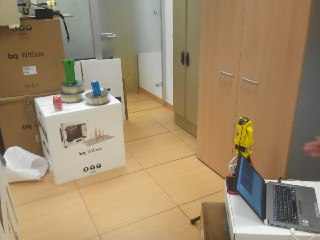
\includegraphics[width=0.65\textwidth]{images/bq.jpg}% 
\caption{Torreta en su entorno de trabajo.}
\label{}
\end{figure}
\FloatBarrier

\newpage

\newpage

\section{Hardware}

El prototipo, representado en la figura \ref{prototipo} consta de cuatro elementos: un ordenador portátil, una webcam, una placa Arduino y una torreta móvil.\\

\begin{figure}[h]
\centering
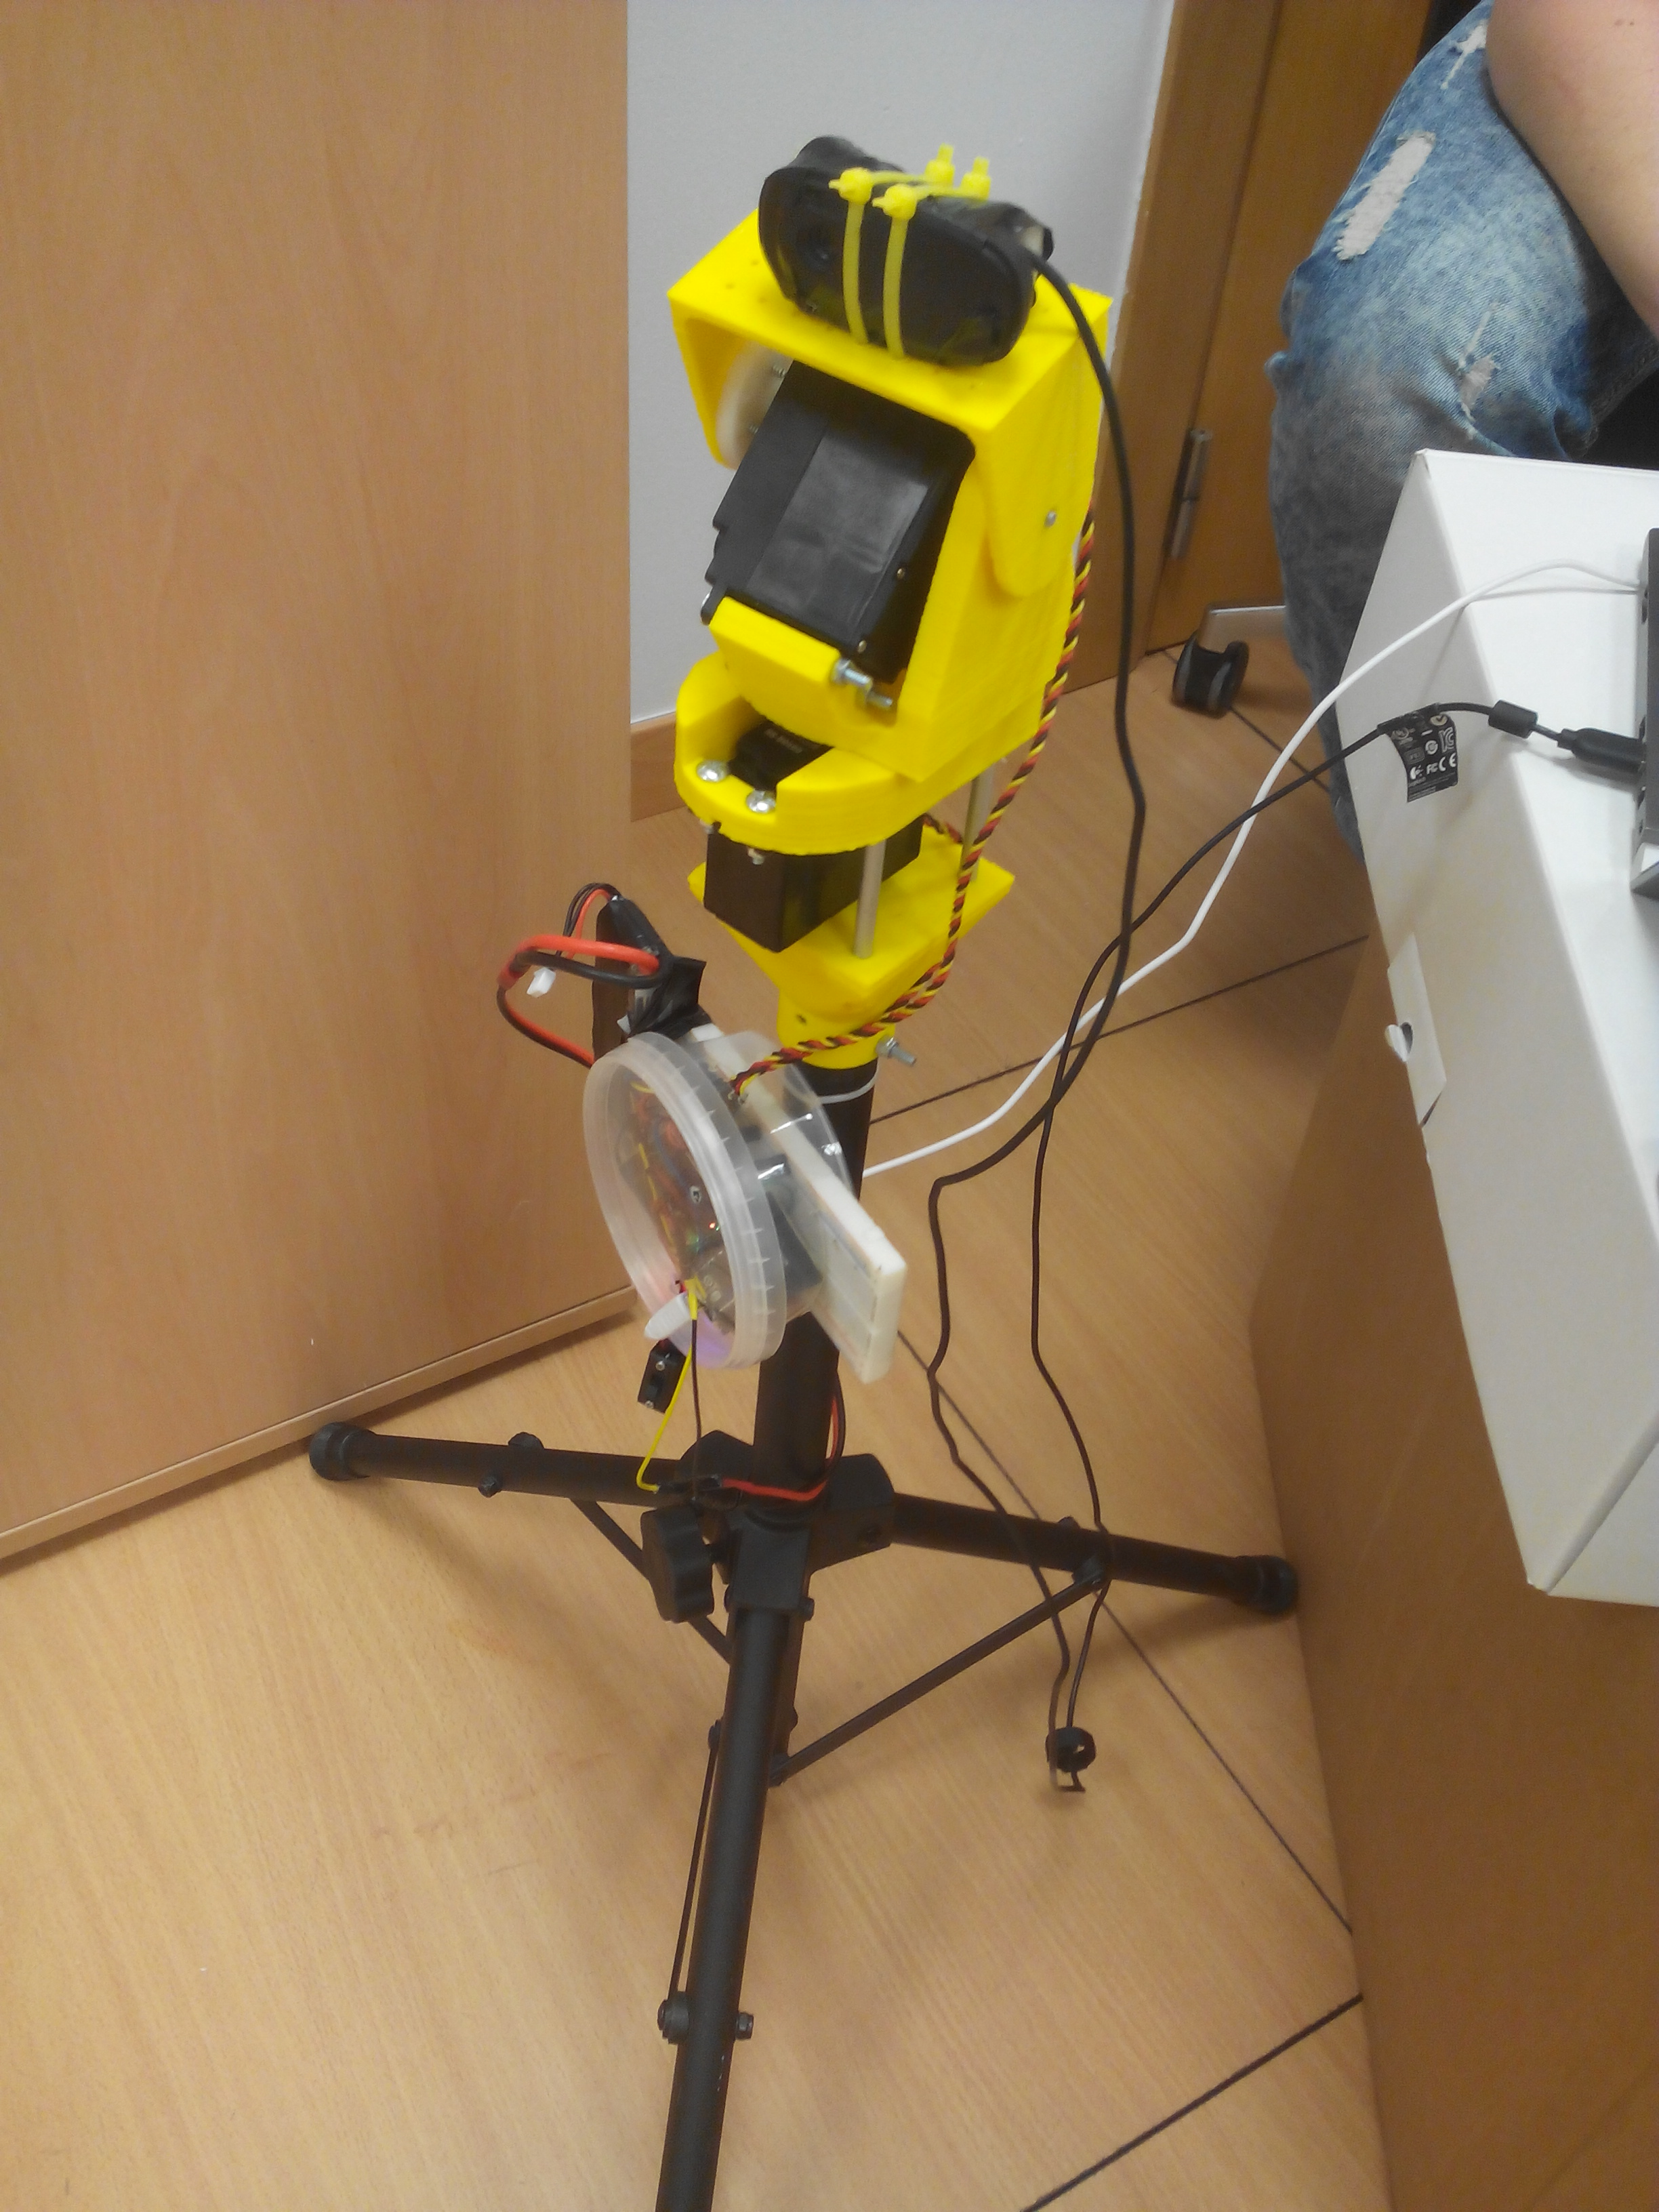
\includegraphics[width=0.35\textwidth]{images/prototipo}% 
\caption{Prototipo realizado.}
\label{prototipo}
\end{figure}
\FloatBarrier

El diseño de la torreta se ha llevado a cabo por medio de programas de diseño CAD como OpenSCAD. OpenSCAD 
\footnote{http://www.openscad.org/} es un programa de diseño orientado a la creación de modelos tridimensionales mediante código. El sistema mecánico consiste en un montaje típico de pan-tilt, accionado mediante servomotores de grandes dimensiones. Sobre la zona móvil de la torreta se ha colocado una webcam. Las piezas diseñadas pueden encontrarse en el repositorio del proyecto\footnote{https://github.com/JavierIH/laserTower}.\\

La fabricación de las piezas de ABS, se ha llevado a cabo mediante la utilización de una impresora 3D doméstica de bajo coste.\\

En cuanto a la electrónica de control, se ha utilizado una placa Arduino para gestionar los movimientos de la torreta. Esta placa, se ha conectado al ordenador por USB. El sistema desarrollado sigue el esquema de la figura \ref{topologia}\\

\begin{figure}[h]
\centering
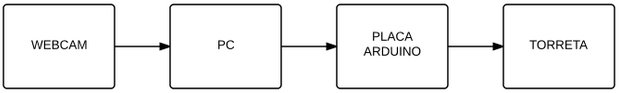
\includegraphics[width=0.85\textwidth]{images/topologia}% 
\caption{Topología del sistema.}
\label{topologia}
\end{figure}
\FloatBarrier

\newpage

\section{Software}
Todo el software de este trabajo se realizó en y para sistemas GNU/Linux. Esta decisión se tomó en base a dos principales razones. La primera, que los sistemas GNU/Linux son de código abierto, lo que facilita el acceso a cualquier persona que lo desee a reproducir este trabajo, estudiarlo y mejorarlo. La segunda, que las herramientas de desarrollo disponibles para GNU/Linux, como CMake\footnote{http://www.kitware.com/opensource/cmake.html} y el compilador gcc, simplifican la configuración y reducen el tiempo de preparación del proyecto respecto a otras alternativas privativas como Visual Studio.\\

Para la realización de este trabajo se han empleado diversas bibliotecas de código libre con el fin de reutilizar código ya existente, reduciendo la carga de trabajo de los autores, y de usar una base de código ya probado que disminuya el número de errores y los acote a nuestro código.\\

El procesado de las imágenes extraídas de la webcam se ha realizado con las bibliotecas OpenCV\footnote{http://opencv.org/}. Estas librerías de código libre, que han sido estudiadas durante esta asignatura, implementan una gran cantidad de algoritmos de visión populares y de uso común, como filtros, detectores de bordes, sustractores de fondo, umbralización, etc. Al disponer de estos algoritmos ya implementados, los autores se pueden centrar  en la creación de aplicaciones que usen dichos algoritmos, aumentando la productividad.\\

El firmware usado en la placa de control de la torreta, la cual está encargada del control de los servomotores que mueven la cámara, usa las bibliotecas Arduino\footnote{http://arduino.cc/}. Arduino incluye un bootloader para facilitar la carga del firmware en el microcontrolador, así como diversas bibliotecas que simplifican tanto el trabajo con los diversos periféricos del microprocesador como el control de los servomotores.\\

La comunicación con la placa de control desde el ordenador encargado del procesamiento de imágenes se llevó a cabo a través de un puerto serie virtual sobre USB. Para poder comunicarse a través de este puerto, se utilizaron las bibliotecas YARP\footnote{http://wiki.icub.org/yarp/}. YARP es un middleware para robots con diversas utilidades para comunicaciones y drivers para distintos periféricos de uso frecuente en robótica, como cámaras, placas de control, motores, sensores, etc. El objetivo de YARP es ofrecer interfaces con las que conseguir un código modular y desacoplado, en el que sea sencillo introducir cambios tanto en el hardware del robot como en su software, y que permita reutilizar el software existente pese a esos cambios.\\

Por último, para la reproducción de sonidos que simulan el disparo de la torreta, se usaron las bibliotecas SDL\footnote{http://www.libsdl.org/} (Simple DirectMedia Layer), que permiten un acceso de bajo nivel a diversos sistemas del ordenador, como gráficos, audio, teclado, ratón, etc.\\

\newpage

\section{Algoritmo de Control}
\subsection{Detección de objetivos}
Para detectar las latas, se han realizado dos algoritmos diferentes: uno basado en el espacio de color RGB y otro en el espacio HSV. Para observar los resultados de ambos algoritmos, se ha utilizado una imagen de prueba como la presentada en la figura \ref{imagendeprueba}\\

\begin{figure}[h]
\centering
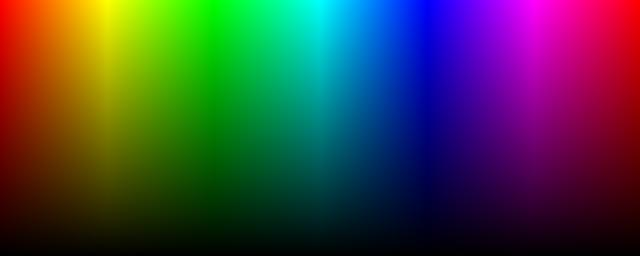
\includegraphics[width=0.7\textwidth]{images/imagendeprueba}% 
\caption{Imagen de prueba}
\label{imagendeprueba}
\end{figure}
\FloatBarrier

El algoritmo de detección basado en RGB se lleva a cabo de la siguiente forma. En primer lugar, se separan los tres canales de la imagen (rojo, verde y azul) en tres imágenes monocanales. Tras esto, se recombinan los canales mediante sumas y restas para obtener las zonas de la imagen que contienen una mayor pureza de color. Por ejemplo, supongamos que queremos realizar una detección del color azul de una imagen. Se tomará como base el canal azul de la imagen y se hallarán las diferencias respecto al resto de componentes de la imagen, realizando la siguiente operación:

\[(AZUL - ROJO) + (AZUL - VERDE)\]

Con este procedimiento, enfrentamos el color azul con el resto de colores de la imagen. Los resultados deben interpretarse como una medida de la pureza del color azul detectada. De este modo, colores que tengan una componente azul muy superior al resto de sus componentes presentarán mayor pureza que otros colores que tengan proporciones similares o superiores del resto de componentes de color frente al azul.\\

Aplicando este algoritmo sobre nuestra imagen de control obtenemos el resultado que puede apreciarse en la figura \ref{rgbazul}\\

\begin{figure}[h]
\centering
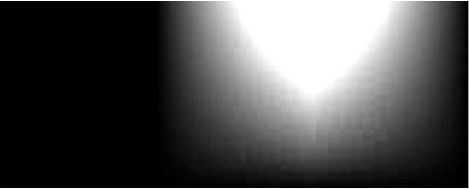
\includegraphics[width=0.7\textwidth]{images/rgbazul}% 
\caption{Detección de color azul en espacio RGB}
\label{rgbazul}
\end{figure}
\FloatBarrier

Una vez obtenido este resultado, podemos realizar una umbralización simple para obtener una imagen binaria que separe nuestro objetivo del entorno. Este método permite la conceptualización del color, no busca la detección de un matiz de color concreto, sino que obtiene como entrada un color (en este caso “azul”) y devuelve un conjunto borroso de colores cercanos a él.\\

Este método puede escalarse a colores no primarios, como por ejemplo el amarillo, obtenido por la suma equitativa de dos colores primarios. Para ello, sumaríamos la pureza de sus dos componentes, rojo y verde; frente a la componente que no forma parte del amarillo, el azul. La fórmula en este caso sería la siguiente:

\[(ROJO - AZUL) + (VERDE - AZUL) \]

Y obtendríamos como resultado la imagen \ref{rgbamarillo}\\

\begin{figure}[h]
\centering
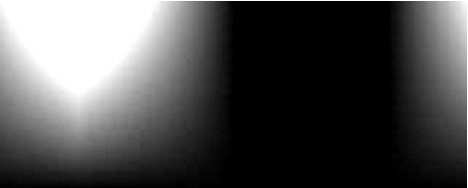
\includegraphics[width=0.7\textwidth]{images/rgbamarillo}% 
\caption{Detección de color amarillo en espacio RGB}
\label{rgbamarillo}
\end{figure}
\FloatBarrier

Sin embargo, es importante recalcar que la búsqueda de colores más complejos incrementa gradualmente la dificultad de los cálculos.\\

El espacio de color HSV también se basa en tres canales diferenciados, pero la codificación de la información es diferente al RGB. Estos tres canales son Hue, Saturation, Value (Matiz o tono, Saturación, Valor). Para esta aplicación, y aprovechando la independencia a la iluminación que ofrece este espacio de color, el principal análisis se hará sobre el canal donde se almacena el color, Hue, dejando en segundo plano los otros dos canales, aunque también se tendrán en cuenta.\\

En primer lugar, es necesario transformar la imagen de un espacio de color al otro para poder trabajar sobre HSV. Para ello se usa la función de OpenCV \textit{cvtColor()} con el código RGB2HSV. Una vez se haya convertido la imagen a HSV, se pueden separar los tres canales donde se almacena la información.\\

Para detectar el color no sólo se debe tener en cuenta el canal H, puesto que los colores gris, blanco y negro también poseen información en este canal y serían detectados como pixeles del color buscado. Para filtrar el gris, blanco y negro, se utilizan los canales restantes. El canal S nos da la saturación de un color. Por ello, si queremos descartar los grises, se ha de colocar un umbral mínimo a partir del cual se deja de encontrar gris en dicho canal. En los extremos del canal V, que representa la intensidad lumínica de los pixeles, se encentran los blancos y los negros. Por ello, para descartarlos se ha de filtrar un rango de valores que no incluya valores en los extremos. \\

Una vez filtrados los grises, blancos y negros, basta con centrarse en en definir en los umbrales superior e inferior en el canal H. Con estos umbrales se podría seleccionar el color con el que se quiera trabajar, sin que interfiera mucho la iluminación del escenario u otros factores.\\

Para programar estos umbrales basta con emplear la función \textit{inRange()}, que permite binarizar una imagen donde los píxeles blancos corresponden a los que las valores de los tres canales que están dentro de los umbrales definidos para cada canal.\\

De este modo, se puede obtener el color que deseemos de un modo sencillo. Por ejemplo, para obtener el color azul basta con definir los umbrales del canal H, como se puede ver en la figura \ref{azulhsv}.\\
\begin{figure}[h]
\centering
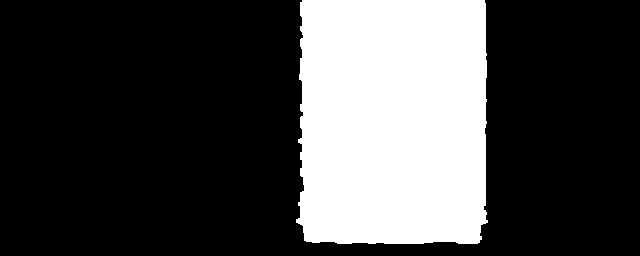
\includegraphics[width=0.7\textwidth]{images/azul.jpg}% 
\caption{Detección del color azul en HSV.}
\label{azulhsv}
\end{figure}
\FloatBarrier
El color más difícil de obtener es el color rojo, ya que está dividido en los extremos del canal H. Para este color en concreto, es necesario repetir el proceso dos veces, una para valores bajos y otra para altos, y aplicar una operación OR de ambas máscaras binarias. De este modo se obtendría las imágenes de la figura \ref{rojohsv}.\

\begin{figure}[h]
\centering
\subfigure[Valores bajos de la componente H.]{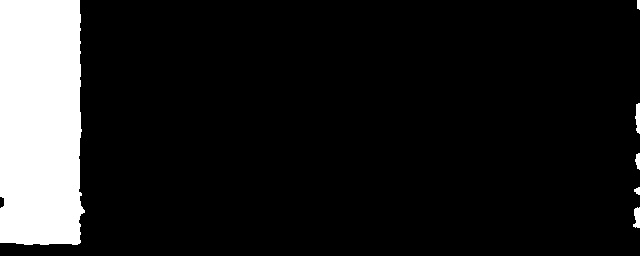
\includegraphics[width=0.35\textwidth]{images/rojo1.jpg} }
\subfigure[Valores altos de la componente H.]{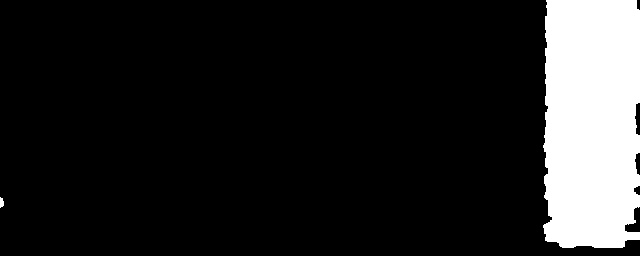
\includegraphics[width=0.35\textwidth]{images/rojo2.jpg} }
\subfigure[OR de ambas máscaras.]{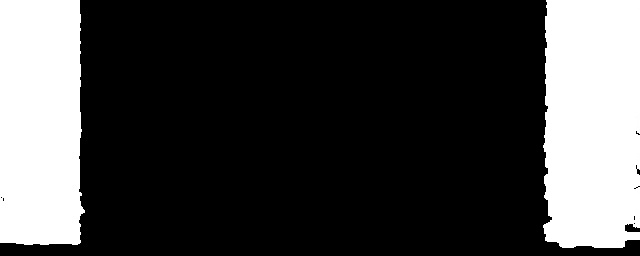
\includegraphics[width=0.7\textwidth]{images/rojo.jpg} }

\caption{Detección del color rojo en HSV.}
\label{rojohsv}
\end{figure} 
\FloatBarrier

Una vez se ha utilizado cualquiera de los dos métodos anteriores, se habrá obtenido una imagen binaria en la que el objetivo es blanco y el fondo es negro. En la figura \ref{binaria} puede observarse un ejemplo.\\

\begin{figure}[h]
\centering
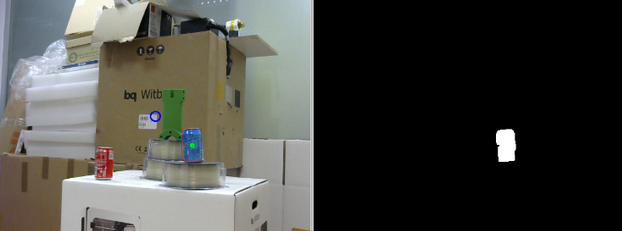
\includegraphics[width=0.9\textwidth]{images/binaria}% 
\caption{Binarización de imagen sobre segmentación de color azul}
\label{binaria}
\end{figure}
\FloatBarrier

Para extraer los datos del objetivo detectado se ha relizado una detección de contornos. Sobre el contorno extraído y teniendo en cuenta que los objetivos a localizar son latas (es decir, objetivos rectangulares), se ha calculado el bounding box del cuerpo del objeto y se han comprobado sus proporciones. Una vez hallado el rectágulo definido por el bounding box, utilizaremos las coordenadas de su centro como el objetivo de la torreta.

\subsection{Visual Servoing}
Tras obtener la posición dentro de la imagen del centroide del objeto, el siguiente paso es dirigir la cámara hacia el objeto. Al representar el centro de la imagen el punto en el que la torreta está apuntando, si se consigue central el objeto en la imagen observada la torreta estará apuntando al objeto. Una mirilla virtual es superpuesta a la imagen como indicador visual de este hecho.\\

Para conseguir centrar al objeto en nuestra imagen, se necesita comandar los dos motores que muevan la cámara. Para cerrar el lazo de control de los motores se utiliza la visión por computador, lo que se conoce como Visual Servoing.\\

El Visual Servoing, tal y como se encuentra en la literatura, conlleva matemáticas complejas, incluyendo una jacobiana visual, que no eran el objetivo de este trabajo. Por ello, se simplificó el problema, controlando la posición de los servos de la torreta en base a la distancia del objetivo al centro de la imagen. En el centro de la imagen se encuentra la mirilla virtual, por lo que cuando el objeto se encuentre en el centro de la imagen, estará dentro del alcance de la torreta.\\

Un sencillo control proporcional para cada eje fue implementado, usando esa distancia al centro de la imagen como error, siguiendo las fórmulas:

\[\Delta X=k_{px} \cdot (X_{objeto}-X_{centro})\] 
\[\Delta Y=k_{py} \cdot (Y_{objeto}-Y_{centro})\]

\subsection{Filtrado}
Debido a las vibraciones producidas al estar la torreta en movimiento, y también a los cambios en la iluminación, la posición del centroide de los objetos puede variar de forma errática. Para un movimiento más suave, se añadió un filtro de Kalman a la posición del centroide de los objetivos, lo que hace que estos cambios erráticos queden filtrados.\\

El filtro de Kalman, además, realiza una estimación del estado del centroide, por lo que si en algún frame capturado el objeto detectado no está (debido, por ejemplo, a una oclusión) o se detecta algún blob de color similar al del objetivo, esta estimación hará que estos errores no influyan tanto durante un breve período de tiempo.\\

\subsection{Medidas de Seguridad}
Para evitar que la torreta pueda disparar en presencia de personas, se diseñó un mecanismo de seguridad simple basado en Cascadas de Haar (Haar-like Feature-based Cascade Classifiers).\\

Las Haar-like Features se obtienen mediante operaciones simples, sumas y restas de intensidades de gris de píxeles, dentro de una ventana deslizante, que sirven como características débiles de la imagen. 
A continuación, una serie de clasificadores colocados en cascada (Adaboost) toman esas características débiles y las organizan de tal forma que se forme un clasificador mucho más robusto que cada una de las características individuales.\\

Al usar operaciones muy simples, con un bajo coste computacional, este método se puede utilizar para detectar caras en tiempo real en la imagen.\\

\newpage


\section{Resultados}
Se ha conseguido implementar todos los objetivos propuestos. La torreta es capaz de localizar y disparar de forma virtual a los objetivos. El usuario puede definir el orden en la que la torreta dispare a los objetivos diferenciandolos por color.\\

Para la realización de este trabajo se han utilizado conocimientos de diferentes ramas. En primer lugar, el uso de las librerías OpenCV y de varias de sus funciones. Se han utilizado dos espacios de color diferentes para obtener información del entorno de diferentes formas, y el resultado ha sido igual de bueno para ambos casos.\\

La torreta presenta mucha inercia y no existe una pausa justo antes del disparo, por esto la torreta no se detiene en el centroide del objetivo durante unos instantes. Esto hace dar la impresión de que la torreta no acierta en el objetivo pasando simplemente a través él, pero realmente sí lo hace si se observa en la captura del fotograma en el que la torreta simula el disparo.\\

El sistema de seguridad detiene el disparo de la torreta en el momento que encuentra una cara. 
La torreta no disparará hasta que no deje de detectar en la imagen a la persona, pero seguirá recalculando el posicionamiento de los servos para apuntar al objetivo.\\

La comunicación entre los diferentes elementos es estable, permitiendo un uso fluido y continuo del programa pudiendo repetirlo varias veces sin necesidad de reiniciar ningún dispositivo.\\

Para la aplicación real, se ha diseñado las piezas para crear una torreta con dos grados de libertad y poder montar sobre ella una cámara. Además, para dotarla de movimiento controlado, se ha programado un microcontrolador que controla los servos y se comunica con el ordenador. La implementación y funcionalidad de los diferentes elementos del sistema ha sido un éxito.\\

Por lo tanto, se puede considerar que todos los objetivos propuestos al inicio del proyecto se han completado saticfactoriamente.\\



\newpage


\section{Trabajos Futuros}
Para un futuro se puede desarrollar una interfaz gráfica que facilite el uso del programa a usuarios no experimentados.\\

También se puede mejorar el tracking pudiendo mejorar y predecir de forma más exacta la posición del objetivo o poder disparar a objetivos en movimiento. Para esto es necesario desarrollar la jacobiana visual y crear un lazo de control mejor que el actual.\\

Esta torreta o una similar se puede incluir dentro del proyecto Robot Devastation de la asociación de robótica de la universidad ASROB, en la que se pretende hacer un videojuego tipo shooter con robots reales teleoperados a través de un ordenador. Esta torreta se puede utilizar como jugador “bot” si se adaptase a parte de sus software al videojuego.\\

La torreta se queda a la espera hasta que el objetivo entra dentro de su campo de visión para la posición dada de los grados de libertad en ese momento. Se puede crear un pequeño algoritmo que permita a la torreta localizar objetivos dentro de la movilidad de sus servos, generando una búsqueda activa.\\
